\documentclass{article}
\usepackage{tikz}
\usepackage{amsmath}
\usepackage{geometry}
\geometry{margin=1in}

\title{Enhanced Unified Implementation Plan for Autonomous CNC Toolpath System}
\author{M365 Copilot}
\date{\today}

\begin{document}
\maketitle

\section{Source Prompts}
\subsection*{Toolpath Prompt}
\textit{Generate toolpaths for fused cuboids avoiding vertical walls and entering from outside.}

\subsection*{Feeds and Speeds Prompt}
\textit{Select feeds and speeds using practical machining heuristics.}

\subsection*{Factory Simulation Prompt}
\textit{Develop an autonomous multi-machine CNC factory with scheduling, tool tracking, and optimization.}

\section{System Architecture}
\begin{center}
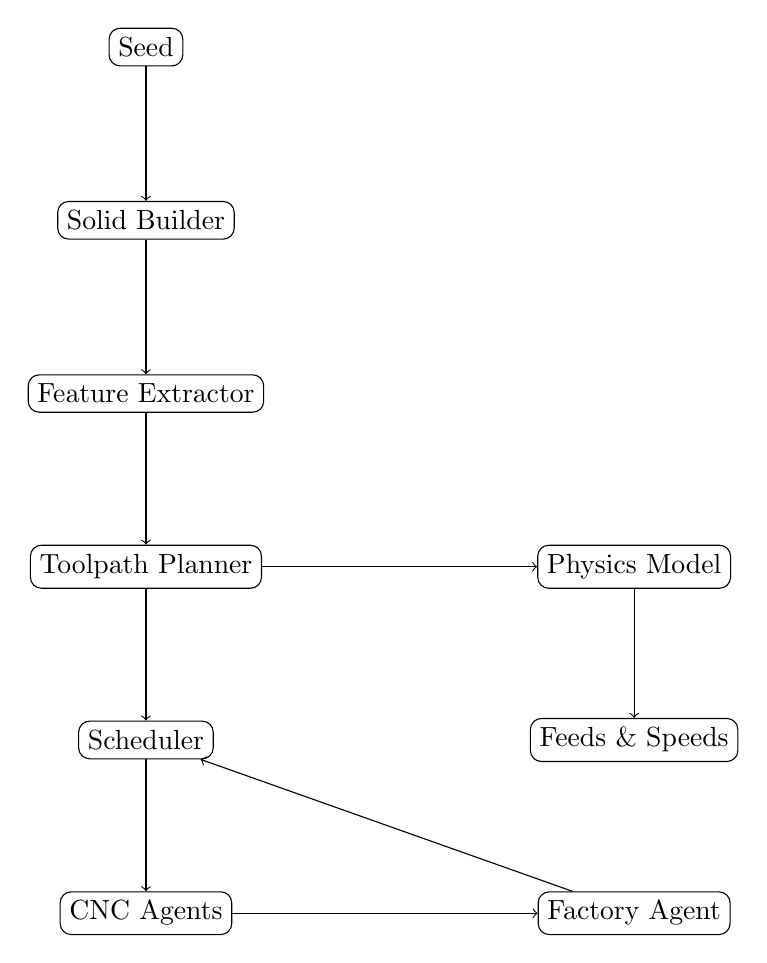
\begin{tikzpicture}[node distance=2.2cm, every node/.style={draw, rectangle, rounded corners}]
\node (seed) {Seed};
\node (solid) [below of=seed] {Solid Builder};
\node (features) [below of=solid] {Feature Extractor};
\node (planner) [below of=features] {Toolpath Planner};
\node (physics) [right of=planner, xshift=4cm] {Physics Model};
\node (fs) [below of=physics] {Feeds \& Speeds};
\node (scheduler) [below of=planner] {Scheduler};
\node (machines) [below of=scheduler] {CNC Agents};
\node (factory) [right of=machines, xshift=4cm] {Factory Agent};

\draw[->] (seed)--(solid);
\draw[->] (solid)--(features);
\draw[->] (features)--(planner);
\draw[->] (planner)--(scheduler);
\draw[->] (scheduler)--(machines);
\draw[->] (planner)--(physics);
\draw[->] (physics)--(fs);
\draw[->] (machines)--(factory);
\draw[->] (factory)--(scheduler);
\end{tikzpicture}
\end{center}

\section{Physics Model Integration}
Cutting force model:
\[
F_c = K_c \cdot A_c
\]
SI: $F_c$ in N, $K_c$ (specific cutting force) in MPa, $A_c$ chip area (mm$^2$)

Power model:
\[
P = \frac{F_c \cdot V}{60}
\]
where $P$ in kW, $V$ in m/min

Torque model:
\[
T = \frac{9550 P}{N}
\]
where $T$ in Nm

Constraint: ensure $P$ and $T$ are below machine limits.

\section{Mathematical Optimization}
Multi-objective cost function:
\[
J = w_1 T_m + w_2 C + w_3 \frac{1}{L} + w_4 S
\]

Where:
\begin{itemize}
\item $T_m$: machining time
\item $C$: cost
\item $L$: tool life
\item $S$: surface finish penalty
\end{itemize}

\section{Tool Crib Management}
- Tool crib resides at factory agent
- Every $\Delta_t = 500$ steps:
\begin{itemize}
\item Query all machines
\item Identify tools with $<20\%$ life
\item Schedule replacement at part change
\end{itemize}

Critical rule:
\begin{itemize}
\item If tool life $<10\%$ $\rightarrow$ immediate machine stop
\end{itemize}

\section{Global Timer System}
Define synchronized clock:
\[
t_{real} = n \cdot t_{unit}
\]
Default: $t_{unit} = 60s$

All agents operate on discrete time steps ensuring concurrency.

\section{Error Handling Architecture}

\subsection{CNC Agent}
- Dashboard with live toolpath
- User prompt box triggers error
- Convert to structured context
- Send to local LLM

Catastrophic condition:
\begin{itemize}
\item Stop machine
\item Send state to factory agent
\end{itemize}

\subsection{Factory Agent}
- Receives error + state
- Converts to LLM prompt
- Evaluates responses
- Selects mitigation strategy
- Sends commands to CNC agent

\section{Improved Modules}

\subsection{Toolpath Planner}
- Safe region computation
- Entry strategies (ramp, helix)

\subsection{Physics-Constrained Feeds}
- Limit feed by power/force

\subsection{Scheduler}
- Uses timer
- Coordinates machine states

\section{Remaining Weaknesses}
\begin{itemize}
\item No full chatter stability model
\item Limited geometry complexity
\item LLM reliability for error recovery unknown
\item No real-time sensor feedback
\end{itemize}

\section{Conclusion}
This improved plan integrates physics, optimization, concurrency, and robust error handling to create a realistic autonomous CNC system.

\end{document}
